\chapter{Аналитический раздел}

\section{Постановка задачи}

В соответствии с заданием на курсовую работу необходимо разработать загружаемый модуль ядра для мониторинга состояния страниц, выделенных процессу.

Для решения поставленной задачи необходимо:

\begin{itemize}
	\item проанализировать структуры и функции ядра, предоставляющие информацию о страницах, выделенных процессу;
	\item разработать алгоритмы и структуру программного обеспечения;
	\item реализовать программное обеспечение;
	\item провести анализ работы разработанного программного обеспечения.
\end{itemize}

\section{Анализ управления памятью}

Операционная система Linux является системой с поддержкой виртуальной памяти. Для каждого процесса создается адресное пространство, которое делится на блоки равного размера, называемые страницами. Размер страницы определяется системно. Единицей деления физической памяти является физическая страница или страничный кадр. При таком механизме организации памяти каждой виртуальной странице ставится в соответствие физический адрес.

Для отображения виртуальной памяти в физическую используются таблицы страницы. Виртуальный адрес разбивается на части: индекс в таблице страниц и смещение. Информация, хранящаяся в элементе таблицы страниц, соответствующем заданному индексу, указывает на адрес физической страницы памяти, в которой хранятся нужные данные. Схема преобразования виртуального адреса в физический адрес показана на рисунке \ref{img:address-translation}.

\begin{figure}[H]
	\begin{center}
		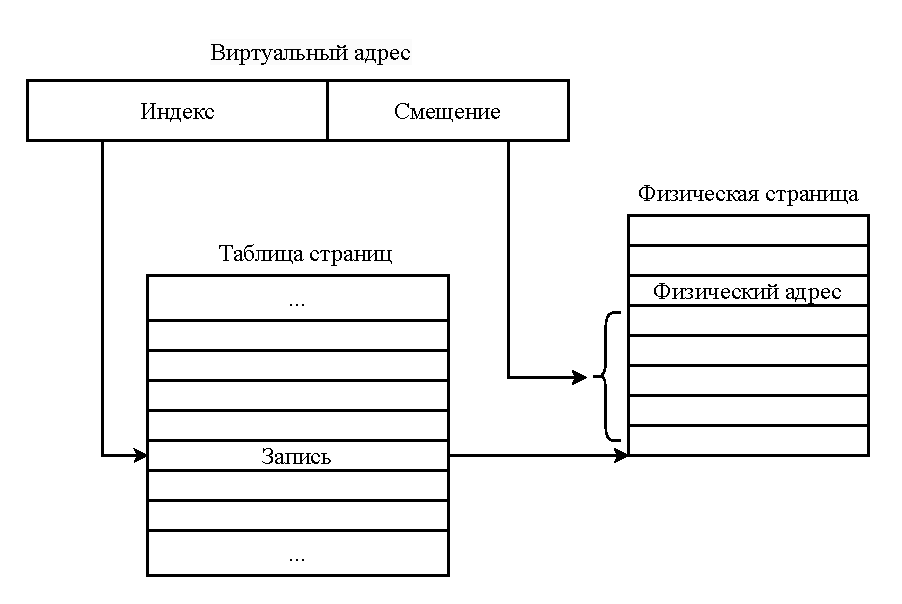
\includegraphics[scale=0.7]{inc/img/address-translation.pdf}
	\end{center}
	\captionsetup{justification=centering}
	\caption{Преобразование виртуального адреса в физический адрес}
	\label{img:address-translation}
\end{figure}
    
Для каждого процесса создается свой набор таблиц страниц. Адресное пространство процесса описывается структурой, называемой дескриптором памяти. В поле pgd дескриптора памяти хранится указатель на глобальный каталог страниц текущего процесса PGD. Элементы в таблице PGD содержат указатели на каталоги страниц среднего уровня PMD. Элементы таблиц PMD содержат указатели на таблицы PTE, записи которой указывают на страницы физической памяти. Связь таблиц страниц представлена на рисунке \ref{img:page-tables}.

\begin{figure}[H]
	\begin{center}
		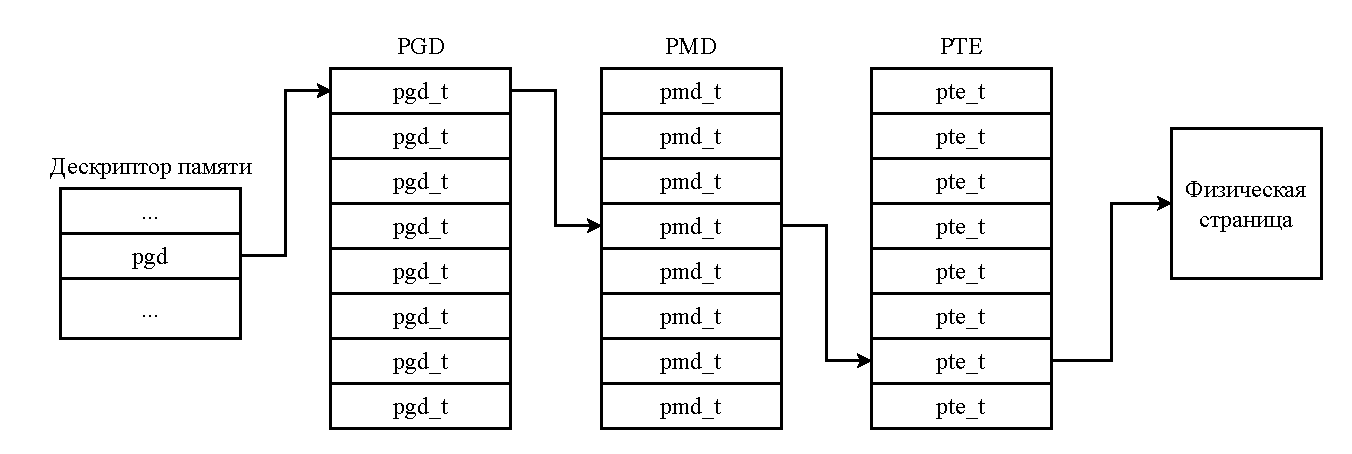
\includegraphics[scale=0.75]{inc/img/page-tables.pdf}
	\end{center}
	\captionsetup{justification=centering}
	\caption{Связь таблиц страниц}
	\label{img:page-tables}
\end{figure}

\section{Анализ структур ядра, предоставляющих информацию о страницах, выделенных процессу}

Для описания процесса в ядре используется структура task\_struct, которая называется дескриптором процесса. Структура описана в файле <linux/sched.h>. Дескриптор процесса позволяет получить информацию о состоянии процесса, открытых файлах и другом. Некоторые поля этой структуры приведены в листинге \ref{lst:task_struct.c}.

\includelistingpretty
    {task_struct.c}
    {C}
    {Структура task\_struct}
    
У объекта task\_struct есть поле mm, содержащее указатель на структуру mm\_struct --- дескриптор памяти процесса. Эта структура описана в файле <linux/mm\_types.h>. Дескриптор памяти процесса предоставляет всю информацию, относящуюся к адресному пространству процесса. Некоторые поля этой структуры показаны в листинге \ref{lst:mm_struct.c}.

\newpage

\includelistingpretty
    {mm_struct.c}
    {C}
    {Структура mm\_struct}
    
Поле mmap объекта mm\_struct содержит указатель на структуру vm\_area\_struct, которая определена в файле <linux/mm\_types.h>. Данная структура используется для описания одной непрерывной области памяти в данном адресном пространстве. Некоторые поля этой структуры представлены в листинге \ref{lst:vm_area_struct.c}.
    
\includelistingpretty
    {vm_area_struct.c}
    {C}
    {Структура vm\_area\_struct}

Каждый дескриптор памяти связан с уникальным диапазоном адресов в адресном пространстве процесса. В поле vm\_start vm\_area\_struct хранится начальный адрес этого диапазона, а в поле vm\_end --- адрес первого байта, расположенного после описываемого диапазона.

В ядре каждая физическая страница памяти представляется в виде структуры page, которая определена в файле <linux/mm\_types.h>. Некоторые поля этой структуры приведены в листинге \ref{lst:page.c}.

\includelistingpretty
    {page.c}
    {C}
    {Структура page}

Для страниц, которые можно сопоставить с пользовательским пространством, в поле \_mapcount объекта page хранится количество записей в таблице страниц, указывающих на данную страницу.

В поле \_refcount объекта page хранится счетчик использования страницы, отражающий количество ссылок в системе на эту страницу. Только что выделенная страница имеет счетчик ссылок, равный 1. Когда счетчик ссылок достигает нуля, страница освобождается.

Для определения счетчика ссылок на страницу используется функция ядра page\_ref\_count, определенная в <linux/page\_ref.h> (листинг \ref{lst:page_ref_count.c}):

\includelistingpretty
    {page_ref_count.c}
    {C}
    {Определение счетчика ссылок на страницу}
    
\section{Использование записей таблицы страниц}

Использование записей таблицы страниц позволяет получить физическую страницу, которая представляется структурой page. Для перемещения по таблицам страниц в файле <asm/pgtable.h> определены следующие функции ядра (листинг \ref{lst:walk_tables.c}):

\includelistingpretty
    {walk_tables.c}
    {C}
    {Перемещение по таблицам страниц}
    
Доступ к физической странице осуществляется следующим образом:

\begin{enumerate}
	\item Системный вызов pgd\_offset() принимает дескриптор памяти процесса и виртуальный адрес и возвращает элемент глобального каталога страниц PGD текущего процесса.
	\item Системный вызов pmd\_offset() запись глобального каталога страниц PGD и виртуальный адрес и возвращает запись каталога страниц среднего уровня PMD.
	\item Системный вызов pte\_offset\_map() принимает элемент каталога страниц среднего уровня PMD и виртуальный адрес и возвращает запись таблицы PTE.
	\item Системный вызов pte\_page() по полученной записи таблицы PTE возвращает объект page.
\end{enumerate}

Функции ядра, представленные в листинге \ref{lst:funcs_node.c}, используются для определения того, существуют ли соответствующие записи таблицы страниц. В случае отстутсвия записи в таблице возвращается 1.
    
\includelistingpretty
    {funcs_node.c}
    {C}
    {Определения счетчика ссылок на страницу}
    
Функции ядра, показанные в листинге \ref{lst:funcs_bad.c}, используются для проверки записей при передаче в качестве входных параметров функциям, которые могут изменить значение записей.
    
\includelistingpretty
    {funcs_bad.c}
    {C}
    {Определения счетчика ссылок на страницу}

\section{Загружаемый модуль ядра}

Ядро операционной системы Linux является монолитным. Это означает, что оно выполняется в общем защищенном адресном пространстве. При реализации микроядра в привилегированном режиме работают только те службы, которым абсолютно необходим привилегированный режим, остальные работают в непривилегированном режиме.

При этом ядро Linux является динамически изменяемым. Это означает, что существует возможность вносить необходимую разработчику функциональность без компиляции ядра. Часть кода, которая может быть добавлена в ядро во время работы, называется модулем ядра. Поддержка модулей позволяет создать минимальное базовое ядро операционной системы, а все дополнительные возможности и драйверы скомпилировать в качестве
загружаемых модулей, т.е. самостоятельных объектов.

\section*{Вывод}
